\chapter{Introdução}\label{chp:introducao}

\section{Processos de Negócio}\label{sec:introducao-processos_negocio}

As organizações, sejam elas de grandes dimensões ou não, são constituídas por recursos humanos e não-humanos que interagem entre si, como por exemplo na troca de informações operacionais entre diferentes áreas de uma empresa. De acordo com a definição apresentada em BPM CBOK\cite{bpm_cbok}, processo é uma agregação de atividades e comportamentos executados por humanos ou máquinas para alcançar um ou mais resultados.

Organizações que adotam processos de negócio bem definidos, estão melhor habilitadas a operar sua rotina e encontram mais facilidade na identificação de pontos de falha, oportunidades de melhorias na execução e planejamento desses processos. Isso acaba por viabilizar o aumento da qualidade na entrega de produtos e serviços para seus clientes ao longo do tempo.

Os processos de negócio, quando realizados de forma desorganizada e despadronizada, levam à ineficiência organizacional pelo simples fato da sua execução não ser otimizada. Isso ocasiona elevação dos custos, aumento no retrabalho, insatisfação dos colaboradores e a consequente diminuição na qualidade dos serviços relacionados. Portanto, torna-se altamente necessário uma boa gestão dos processos, a fim de que esses problemas sejam evitados ou mitigados a tempo e não tornem-se um câncer corporativo. 

\section{Automatização de Processos de Negócio}\label{sec:introducao-automatizacao}

Uma boa gestão de processos busca padronizar as etapas de um processo, e garantir um acesso mais rápido e eficiente às informações, estabelecendo melhores condições para a execução e controle de processos de negócio. Para atingir este objetivo, conta-se com o suporte de sistemas de informação que auxiliem na execução das etapas do processo de acordo com os padrões definidos. Estes sistemas também precisam acompanhar a flexibilidade da constante mudança dos processos, bem como fornecer ferramentas ao gestor para monitorar e controlar os processos, o que termina por aperfeiçoar a tomada de decisão no nível estratégico organizacional.

A automatização de processos de negócio também reduz a dependência de atuação humana na execução de algumas tarefas mecânicas e repetitivas que passam a ser executadas pelos sistemas. No entanto, são raros os casos em que a interação humana é totalmente extinta, sendo necessário uma atenção especial para que essas tarefas sejam executadas da maneira e sequência lógica mais otimizada possível.

\section{Exemplo de Processo de Negócio}\label{sec:introducao-caso_real}

Para ilustrar nossa discussão, descrevemos uma falha real ocorrida em 2013 com uma gigante do mercado de varejo e apresentaremos uma sugestão para o estabelecimento de um processo que busca solucionar, padronizar e controlar a execução dessa atividade para que o mesmo erro não seja observado. Vale notar que sem a adoção de um sistema que automatize a execução das tarefas, é praticamente inviável o correto estabelecimento deste processo.

Em um cenário de operação de um portal de e-commerce é muito importante a gestão dos preços praticados pela empresa nas diferentes categorias que compõem o mix de produtos ofertados ao consumidor. Erros cometidos por uma precificação manual indevida podem levar a altos prejuízos financeiros e ações na justiça por parte dos consumidores, além de afetar a imagem da corporação perante o mercado. 

O caso ocorrido com a gigante Walmart no portal brasileiro em dezembro de 2013, exemplifica bem o cenário descrito no parágrafo anterior. Neste caso, um computador que custava R\$2.398,00 reais foi anunciado por R\$580,00, o que representava um diferença de 75\% a menos em relação ao valor original. Este caso foi noticiado pela imprensa na época, e também houve bastante repercussão nas redes sociais, deixando muitos clientes insatisfeitos pelo cancelamento da compra\cite{noticia_erro_walmart}. 

Nesse caso, torna-se necessária a implantação de um processo de precificação manual que envolva a avaliação de regras que limitem a troca de preço sem a aprovação de alçadas superiores. Essa nova gestão tem por objetivo trazer mais qualidade e segurança nas mudanças de preço solicitadas pelos diferentes precificadores das categorias do site, alinhando assim a gestão de preços do portal e evitando trocas de preço equivocadas ou não autorizadas pelos gestores.

O processo inicia com a decisão do analista de uma determinada categoria de produtos do site pela mudança de preço de um produto. O novo preço do produto é definido pelo analista e enviado para aprovação.

A solicitação enviada pelo analista é avaliada quanto a regra de alçada definida pelos gestores. Caso possua uma variação de preço acima de 30\%,  por exemplo, deverá passar pela aprovação de dois gestores. Em um cenário real de negócios, certamente a regra seria mais complexa, como por exemplo variando em função da categoria do produto. Entretanto, assumiremos a regra da variação de 30\% nas demonstrações como forma de simplificar o entendimento e aplicação das regras de negócio estabelecidas para o processo.

Após a avaliação da variação de preço, caso tenha sido acima de 30\%, o processo deve ser encaminhado para a aprovação de dois gestores. Caso a variação seja menor ou igual a 30\%, a mudança não requer aprovação. Após isso, a troca de preço será efetuada no portal.

A Figura \ref{fig:exemplo_bpmn-problema} descreve de forma visual o fluxo do processo descrito anteriormente:

\begin{figure}[H]
  \centering
  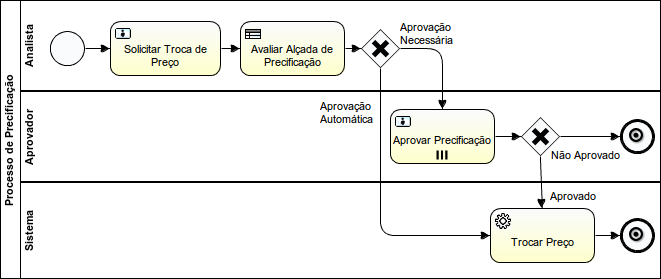
\includegraphics[width=1.0\textwidth]{imagens/ProcessoDePrecificacao.png}
  \caption{Processo de Precificação Manual}
  \label{fig:exemplo_bpmn-problema}
\end{figure}

\section{Solução para Automatização e Gestão de Processos}\label{sec:introducao-ferramenta}

Os sistemas de BPM\cite{bpm}, conhecidos como BPMS\cite{bpms}, possibilitam a implementação de estratégias de operacionalização organizacional por meio de processos, fazendo uso de motores de automação e ferramentas que suportam o ciclo de vida dos processos. Melhorias na visibilidade da operação, facilidades para medir e controlar as etapas de um processo através de sua padronização, adoção de tecnologias de integração de sistemas e automatização de tarefas repetitivas são alguns dos pontos positivos identificados com a adoção desse tipo de solução.  

A adoção de soluções BPM trazem também alguns desafios. Por se tratarem de sistema robustos desenvolvidos para gerenciar processos complexos, sua implantação e manutenção demandam um alto custo: mudanças nos processos irão exigir adaptações nas soluções implantadas, o que pode demandar alto custo e tempo; processos podem ter sua execução impactada devido a situações não previstas durante sua modelagem; além disso da manutenção de profissionais capacitados para gerenciar e suportar essa nova estrutura tecnológica. Portanto, é necessária uma avaliação criteriosa para que a implantação e automatização seja feita na medida correta.

Considerando a complexidade na adoção de ferramentas BPMS\cite{bpms} para a gestão e automatização de processos, buscamos uma alternativa capaz de suprir e contemplar fluxos de trabalho menos complexos, garantindo um nível satisfatório de gestão e automação de processos comuns em ambientes corporativos. Essa ferramenta deveria ser de rápida implantação, simples configuração, possuir uma interface amigável com os atores do processo, e possibilitar rápidas customizações no fluxo de trabalho, garantindo assim certo nível de flexibilidade a mudanças.

Para suprir esta demanda, propomos a utilização do Redmine, ferramenta open-source criada inicialmente para a gestão de projetos. Apesar de não ser o objetivo para o qual foi criado, o Redmine se mostra bastante aplicável para a gestão de processos quando consideramos os recursos oferecidos pelo módulo de gerenciamento de tarefas, os quais seguem um fluxo configurável, bem parecido com os fluxos de processos. As possibilidades de cadastrar campos personalizados e de desenvolver novos plugins também contribuem significantemente para que este software se encaixe bastante bem como gestor de processos em contextos com processos simples e que dependem da interação de pessoas. Ressalta-se ainda o baixo custo de implantação para automatização de processos e a possibilidade de manutenção dos fluxos de trabalho por usuários sem experiência com programação, que encontra-se no Redmine.

Entretanto, a utilização do Redmine como gerenciador de processos mostra-se limitada quando a demanda é automatizar um processo um pouco mais complexo, com a ocorrência de fluxos paralelos, ou a automatização de etapas por outros sistemas.

Com o objetivo de estender o Redmine para o atendimento de fluxos de trabalho mais complexos, identificamos a necessidade do desenvolvimento de um motor de processos mais robusto que possibilitasse novas opções e configurações de fluxos na ferramenta. Entretanto, ao avaliarmos a quantidade de possibilidades de fluxos, o desenvolvimento de uma solução desse porte acabou por convergir com soluções praticadas por ferramentas BPMS\cite{bpms}. 

Nesse sentido, torna-se interessante propor uma solução integrada que aproveite a capacidade de modelagem e automatização de fluxos complexos de um BPMS\cite{bpms}. Uma interface amigável e customizável ao usuário provida pelo Redmine. Nasce assim, a ideia de propor a integração do Redmine com um BPMS\cite{bpms}. A capacidade de extensão e desenvolvimento de novas funcionalidades do Redmine abriu portas para esta ideia. Alia-se a isto, o fato de que a maioria dos BPMS\cite{bpms} possuem APIs\cite{api} bem documentadas para integração com outros sistemas.

Para esta integração com o Redmine, buscamos um BPMS\cite{bpms} que atendesse a determinados critérios. Esta ferramenta deveria ser gratuita, de código-fonte aberto, leve, extensível, contar com uma API\cite{api} REST\cite{rest} de fácil integração e possuir uma boa documentação. Ao avaliar as opções disponíveis, identificamos uma ferramenta que se encaixava bastante bem nos critérios adotados: o Activiti BPM. O Activiti BPM é desenvolvido na linguagem de programação Java\cite{java-history} e é facilmente integrável com aplicações existentes por sua leveza e API\cite{api} amigável, além de utilizar a notação BPMN 2.0\cite{bpmn20} para a modelagem dos processos.

Como principal desafio desta proposta de uma ferramenta integrada de automatização e gestão de processos, identificamos a definição de um modelo de execução que fosse capaz de aliar o benefício de ambas as plataformas, sem acrescentar muita complexidade durante a implantação de uma solução deste porte. Além disso, o desafio da sincronização de dados e estados entre as ferramentas também assumiu papel fundamental nas decisões de modelagem durante o desenvolvimento desta integração.


\section{Organização do Texto}\label{sec:introducao-organizacao_texto}

O restante deste texto está organizado da seguinte forma: 

No capítulo 2 apresentamos como o Redmine pode ser utilizado como gestor de processos. No capítulo 3 introduzimos informações importantes sobre o contexto de gestão de processos de negócio. No capítulo 4 detalhamos a solução proposta para automatização de processos de negócio complexos através da integração do Redmine com um sistema de gerenciamento de processos. No capítulo 5 avaliamos a proposta apresentada e discutimos melhorias futuras. No capítulo 6 apresentamos as conclusões do trabalho.